\chapter{Towards new physics: $R_H$}
\label{sec:RKst_theory}

Flavor-Changing Neutral Currents (FCNCs) processes, where a quark changes its flavour without altering its 
electric charge, are forbidden in the SM at tree level and arise only at one loop, typically by the exchange 
of a W boson. Hence, they are sensitive to quantum corrections by loops of heavy particles at and above the 
electroweak scale ($\sim 100$ GeV). The rare decays $b \rightarrow s \gamma $, $b \rightarrow s g$, 
$b \rightarrow s \ell^+\ell^-$, where $l =  e \text{ or } \mu$, are good probes for these processes. 
In particular, in this work, decays of $b \rightarrow s\mumu (\ee)$ type, are considered. These decays happen 
through loop diagrams, called ``penguins diagrams". Fig.~\ref{fig:RKpenguins} shows the possible Feynman diagrams 
producing semileptonic $\Bz \to K/\Kstar\ell^+\ell^-$ decays while Fig.~\ref{fig:NPpenguins} shows how the Feynman 
diagrams of these processes may include new particles and therefore be used to probe new physics. 
A series of recent LHCb measurements \cite{TomRDreview} shows tensions with SM predictions, which makes it
interesting to further investigate these processes.

%Recently 
%the measurement of the $B_s \rightarrow \mu^+ \mu^-$ branching fraction by the LHCb experiment has not shown 
%any deviations from the SM \cite{LHCb-PAPER-2012-007}.

\begin{figure}[h]
\centering 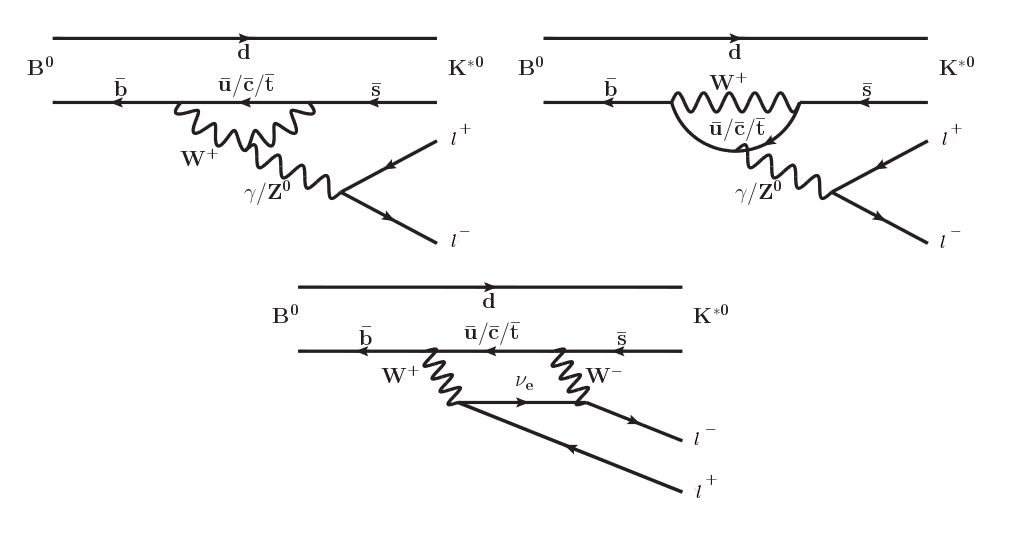
\includegraphics[width=0.8\textwidth]{RKst/figs/penguins3.png}
\caption{Loop diagrams of the $B_d \rightarrow K/K^{*0}l^+l^-$ process.}
\label{fig:RKpenguins}
\end{figure}

In order to exploit the sensitivity of loop diagrams, in 2004 Hiller and Kruger proposed the measurement 
of the $R_H$ ratio \cite{Hiller:2003js}, defined in Eq. \ref{eqRX}, where $H$ can be an inclusive state containing 
an $s$ quark ($X_s$) or an s-quark resonance like $K$ or $\Kstar$.
\begin{equation}
\label{eqRX}
R_{K^{*0}} = \frac{\int_{4m_{\mu^2}} \frac{ d\BR(\Bz \to \Kstar\mumu) }{ds}}{ \int_{4m_{\mu^2}}\frac{ d\BR(\Bz \to \Kstar\ee) }{ds}} ds
\end{equation}
In this quantity the decay width is integrated over the squared dilepton mass, $s = q^2$, starting from 
$s_{min} = 4m_{\mu}$, which is the threshold for the $\mu\mu$ process, up to $s_{max} = m_b^2$. 
The notation $\BR(X \rightarrow ~final ~state)$ denotes the fraction of $X$ particles which decays in the 
given final state, this is called ``branching ratio". For example $\BR(\Bz\to\Kstar\mumu)$ is the
fraction of \Bz particles which decays into $\Kstar\mumu$ with respect to all allowed \Bz decays.

The advantage of using these observables is that, in the theoretical prediction, hadronic uncertainties 
cancel out. Furthermore, experimentally, some of the systematics also cancel out in the ratio giving a better 
measurement. For example, what is measured is the number of $\mu\mu$ and $ee$ decays which happen in a 
certain period of time and then the luminosity ($\mathcal{L}$) is used to obtain a cross section ($\sigma$), 
using $R = \mathcal{L}\sigma$, where $R$ is the rate with which a decay happens. The luminosity measurement
is usually a source of systematic uncertainty, however it appears on both sides of the ratio
and therefore cancels out.

\begin{figure}[h]
\centering 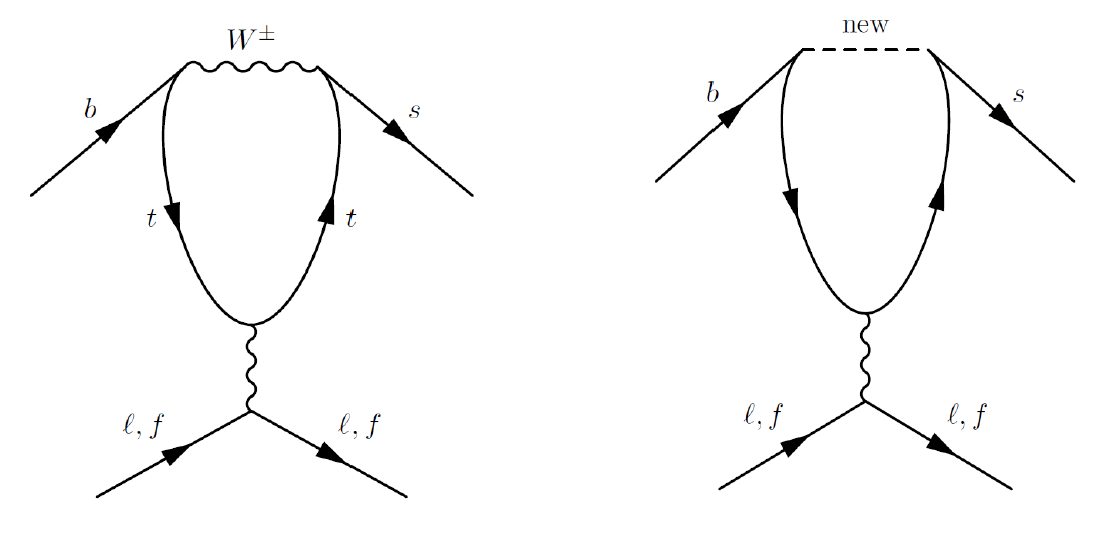
\includegraphics[width=0.8\textwidth]{RKst/figs/penguins.png}
\caption{Example of penguin diagrams, on the left involving SM particles and on the right 
involving new possible particles.}
\label{fig:NPpenguins}
\end{figure}

Since the Standard Model does not distinguish between leptons the predicted value for this ratio 
is $R_H = 1$ for massless leptons. Taking effects of order $m_\mu^2 / m_b^2$ into account Hiller
and Kruger calculate that in the SM~\cite{Hiller:2003js} and in the full \qsq range:

\begin{equation}
\begin{array}{l}
R_{X_s} = 0.987 \pm 0.006 \\
R_K = 1.0000 \pm 0.0001 \\
R_{\Kstar} = 0.991 \pm 0.002
\end{array}
\end{equation}

Under the assumptions:

\begin{itemize}
\item right-handed currents are negligible;
\item (pseudo-)scalar couplings are proportional to the lepton mass;
\item there are no CP-violating phases beyond the SM.
\end{itemize}

The measurement of the $R_H$ ratios is of particular interest after the recent
measurement of the branching ratio of the $\Bs\to\mumu$ decay~\cite{CMS:2014xfa} where no
evidence of NP was found. In fact the quantities $R_H - 1$ and
$\BR(\Bs \to \mumu)$ remain proportional with
%
\begin{equation}
\frac{R_H - 1}{\BR(\Bs \to \mumu)} \sim 2 \cdot 10^{-5}
\end{equation}
%
A joint measurement of this two quantities can give much information and constrain MFV models.
If $R_X = 1$ and $\BR(\Bs \to \mumu)$ is close to the SM prediction as it is measured to be
this will allow to put strong constraints on extensions of the SM.
If instead $R_H > 1$ and the equation above is not verified, this would mean that one of the
assumptions listed above are not verified, which can happen is some extensions of the SM,
for example Super-Symmetric models with broken R-parity.

\subsection{Experimental status}

The $R_K$ and $R_{\Kstar}$ have already been measured at the B-factories (hence in $e^+e^-$ collisions).
And the $R_K$ ratio has been also recently measured at LHCb~\cite{LHCb-PAPER-2014-024} in the $1 < \qsq < 6$ \gevgevcccc,
which provided the currently most precise measurement. This measurement showed a 2.6$\sigma$
deviation from the SM prediction. 
The experimental status is summarised in Tab.~\ref{expstatus}. As for $R_K$ LHCb is expected
to reduce the error on $R_{\Kstar}$ by at least a factor of 2 with respect to the B-factories.

\begin{center}
\begin{table}[h!]
\label{expstatus}
\centering
\begin{tabular}{c|c|c|c}
 	& Belle 			& BaBar 		& LHCb \\
 \hline
$R_K$			& $1.06 \pm 0.48 \pm 0.05$	& $1.38^{+0.39+0.06}_{-0.41-0.07}$ & $0.745^{+0.090}_{-0.074} \pm 0.036$\\
$R_{\Kstar}$	& $0.93 \pm 0.46 \pm 0.12$	& $0.98^{+0.30+0.08}_{-0.31-0.08}$ & --\\
\end{tabular}
\caption{Previous $R_X$ measurement by the BaBar~\cite{Lees:2012tva} and Belle~\cite{Wei:2009zv} experiment.}
\end{table}
\end{center}

\section{The $R_{\Kstar}$ analysis}

The aim of this analysis is to measure the $R_{\Kstar}$ using $p-p$ collision data collected by the LHCb
detector in 2011 and 2012, corresponding to 3 \invfb of integrated luminosity.
In order to do this $\Bz \to \Kstar\mumu$ and $\Bz \to \Kstar\ee$ (``rare channels") candidates are
reconstructed. In both cases $\Kstar$ is reconstructed through its decay in a kaon and a pion of opposite signs.

The analysis has to separate signal candidates from background candidates which have similar observed properties. 
The selection presented in Sec. \ref{sec:RKst_selection} aims to maximise the yield while minimising
the background contamination. Two types of backgrounds are identified: ``peaking background" and ``combinatorial background". 
The first comes from the mis-reconstruction of other decays or from partially reconstructed events. This type 
of background,  because its specific kinematic properties, usually peaks in some variable, such as the invariant
mass of all final particles, therefore we can remove these events by removing the peak. The combinatorial background 
instead comes from the random combination of particles and can be lowered selecting events with good-quality tracks 
and vertices.

Together with the rare channels the decays reaching the same final states via a \jpsi
resonance, $\Bz\to\Kstar\jpsi(\to\ell^+\ell^-)$, are also reconstructed and referred as
``charmonium" or ``resonant" channels. These decays have identical final states to the rare channels, differing
only in the invariant mass of the dilepton pair. As they have much higher statistics they can be used as
control samples. 

In Sec.~\ref{sec:Rkst_efficiency} the efficiency of selecting and reconstructing each channel is extracted
and, finally, in Sec.~\ref{sec:RKst_result} the $R_{\Kstar}$ ratio defined is built as the double ratio
of rare and resonant channels:

\begin{equation}
R_{\Kstar} = 
 \frac{N_{\Bz\to\Kstar ee}}{N_{\Bz\to\Kstar\jpsi\to ee}} 
\cdot \frac{N_{\Bz\to\Kstar \jpsi \mumu}}{N_{\Bz\to\Kstar\mumu}}
\cdot \frac{\varepsilon_{\Bz\to\Kstar \jpsi \to ee}}{\varepsilon_{\Bz\to\Kstar ee}} 
\cdot \frac{\varepsilon_{\Bz\to\Kstar \mumu}}{\varepsilon_{\Bz\to\Kstar\jpsi\to \mumu}}
\end{equation}

As no new physics is expected to affect charmonium resonances the ratio of the \jpsi channels
is 1 and therefore $R_{\Kstar}^{'} = R_{\Kstar} \times R_{\jpsi} = R_{\Kstar}$.
On the other hand using the relative efficiencies between the rare and resonant channels
allows to cancel out many effects resulting in a better control of systematic uncertainties.  


%\subsection{Data and Monte Carlo samples}

%This analysis is based on a data set corresponding to $3 \fb$ of integrated luminosity collected by the
%LHCb detector in 2011 and 2012.
%Candidates have been reconstructed with the ``Reco14" version of the reconstruction software.%

%\begin{table}[h!]
%\label{TabMC}
%\begin{center}
%\begin{tabular}{c|c|c}
% Sample					& {$N_{gen}$}		& Br \\ \hline
%$B^0 \rightarrow K^{*0} \mu\mu$		&	519496		& $1.05 \cdot 10^{-6}$  \\
%$B^0 \rightarrow K^{*0} J/\psi$		&	518996		& $1.34 \cdot 10^{-3}$    \\
%$B_s \rightarrow \phi \mu\mu$ 		&   	512995		& $1.23 \cdot 10^{-6}$    \\
%$B^+ \rightarrow K \mu\mu$ 		&    	519999		& $4.8 \cdot 10^{-7}$  \\
%$B^0 \rightarrow K^{*0} ee$		&    	6006968		& $1.05 \cdot 10^{-6}$   \\
%$B^0 \rightarrow K^{*0} \gamma$ 	&   	7413465		& $4.33 \cdot 10^{-5}$   \\
%$J/\psi \rightarrow ll$			&   			& $5.93 \cdot 10^{-2}$    \\
%$\phi \rightarrow KK$ 			&   			& $0.489$    \\
%\end{tabular}
%\caption{Summary of the Monte Carlo samples used for the analysis together with the branching fractions of
%the simulated processes.}
%\end{center}
%\end{table}

%In order to study the peaking background properties, our cuts efficiency and to train the multivariate analysis
%we also used Monte Carlo events from the MC11a production. Events are fully simulated in the detector and
%reconstructed using the same algorithms as for data. In Table \ref{TabMC} are reported the MC samples used
%together with the number of generated events and the branching fractions of the simulated processes



